\section{Results and Discussion}

\subsection{Experimental Setup}
\noindent\hspace*{\parindent} Describe your experimental setup, dataset, or simulation environment here.

\subsection{Results}
\noindent\hspace*{\parindent} Present your results here, referring to figures and tables as needed, e.g. see Figure~\ref{fig:results-example} and Table~\ref{table:results-example}.

\begin{figure}[H]
    \centering
    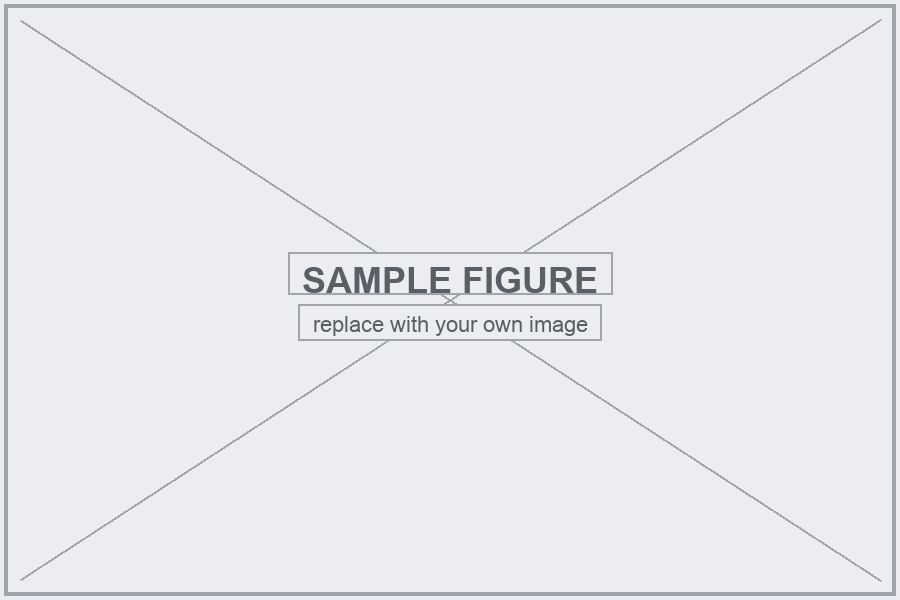
\includegraphics[width=0.6\textwidth]{figure/sample-figure.png}
    \caption{Example results figure -- replace with your own plot}
    \label{fig:results-example}
\end{figure}

\begin{table}[H]
    \centering
    \caption{Example results comparison}
    \begin{tabular}{|c|c|c|}
    \hline
    \textbf{Method} & \textbf{Metric A} & \textbf{Metric B} \\
    \hline
    Baseline & $0.00$ & $0.00$ \\
    \hline
    Proposed & $0.00$ & $0.00$ \\
    \hline
    \end{tabular}
    \label{table:results-example}
\end{table}

\subsection{Discussion}
\noindent\hspace*{\parindent} Interpret your results here: what do they mean, how do they compare to prior work (cite as needed, e.g. \cite{Salzmann_2023}), and what are the limitations?
